    \section{Módulo de um número real}

    \noindent
	\textbf{Definição:} Seja $x$ um número real. O módulo de $x$, denotado por $|x|$, é definido como:

     \begin{tcolorbox}[colback=white,colframe=minha_cor,coltitle=black,title=Definição: Módulo de número real] 
        \[
        {|x| = \left\{  
	       \begin{array}{c}
		     \;\; x \;\;\; \text{se} \;\;\; x \ge 0\\
		     -x \;\;\; \text{se} \;\;\; x < 0\\
	       \end{array} 
	       \right.
        }
        \]
        \end{tcolorbox}
        
	   Em uma representação geométrica, tem-se que:\\
 
		Se $x \le 0$ então:
		\begin{center}
		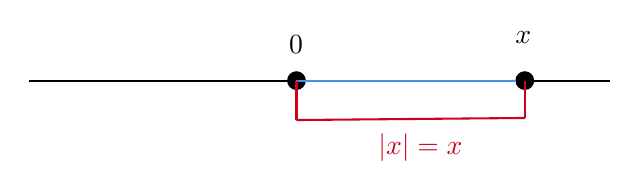
\begin{tikzpicture}[x=0.75pt,y=0.75pt,yscale=-1,xscale=1]
			\draw    (431,82) -- (472,82) ;
			\draw  [fill={rgb, 255:red, 0; green, 0; blue, 0 }  ,fill opacity=1 ] (317,82) .. controls (317,79.79) and (318.79,78) .. (321,78) .. controls (323.21,78) and (325,79.79) .. (325,82) .. controls (325,84.21) and (323.21,86) .. (321,86) .. controls (318.79,86) and (317,84.21) .. (317,82) -- cycle ;
			\draw  [fill={rgb, 255:red, 0; green, 0; blue, 0 }  ,fill opacity=1 ] (427,82) .. controls (427,79.79) and (428.79,78) .. (431,78) .. controls (433.21,78) and (435,79.79) .. (435,82) .. controls (435,84.21) and (433.21,86) .. (431,86) .. controls (428.79,86) and (427,84.21) .. (427,82) -- cycle ;
			\draw    (192,82) -- (321,82) ;
			\draw [color={rgb, 255:red, 74; green, 144; blue, 226 }  ,draw opacity=1 ]   (321,82) -- (427,82) ;
			\draw [color={rgb, 255:red, 208; green, 2; blue, 27 }  ,draw opacity=1 ]   (321,82) -- (321,101) ;
			\draw [color={rgb, 255:red, 208; green, 2; blue, 27 }  ,draw opacity=1 ]   (321,101) -- (431,100) ;
			\draw [color={rgb, 255:red, 208; green, 2; blue, 27 }  ,draw opacity=1 ]   (431,82) -- (431,100) ;
			\draw (359,106) node [anchor=north west][inner sep=0.75pt] [color={rgb, 255:red, 208; green, 2; blue, 27 }  ,opacity=1 ] [align=left] {$|x| = x$};
			\draw (316,59) node [anchor=north west][inner sep=0.75pt]   [align=left] {$0$};
			\draw (425,57) node [anchor=north west][inner sep=0.75pt]   [align=left] {$x$};
		\end{tikzpicture}
            \end{center}
            
		Se $x \ge 0$ então:    
            \begin{center}
		\tikzset{every picture/.style={line width=0.75pt}}
		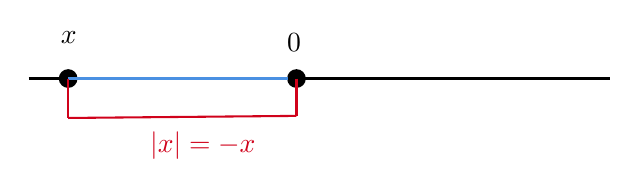
\begin{tikzpicture}[x=0.75pt,y=0.75pt,yscale=-1,xscale=1]
			\draw    (321,82) -- (472,82) ;
			\draw  [fill={rgb, 255:red, 0; green, 0; blue, 0 }  ,fill opacity=1 ] (207,82) .. controls (207,79.79) and (208.79,78) .. (211,78) .. controls (213.21,78) and (215,79.79) .. (215,82) .. controls (215,84.21) and (213.21,86) .. (211,86) .. controls (208.79,86) and (207,84.21) .. (207,82) -- cycle ;
			\draw  [fill={rgb, 255:red, 0; green, 0; blue, 0 }  ,fill opacity=1 ] (317,82) .. controls (317,79.79) and (318.79,78) .. (321,78) .. controls (323.21,78) and (325,79.79) .. (325,82) .. controls (325,84.21) and (323.21,86) .. (321,86) .. controls (318.79,86) and (317,84.21) .. (317,82) -- cycle ;
			\draw    (192,82) -- (211,82) ;
			\draw [color={rgb, 255:red, 74; green, 144; blue, 226 }  ,draw opacity=1 ]   (211,82) -- (317,82) ;
			\draw [color={rgb, 255:red, 208; green, 2; blue, 27 }  ,draw opacity=1 ]   (211,82) -- (211,101) ;
			\draw [color={rgb, 255:red, 208; green, 2; blue, 27 }  ,draw opacity=1 ]   (211,101) -- (321,100) ;
			\draw [color={rgb, 255:red, 208; green, 2; blue, 27 }  ,draw opacity=1 ]   (321,82) -- (321,100) ;
			\draw (249,106) node [anchor=north west][inner sep=0.75pt]  [color={rgb, 255:red, 208; green, 2; blue, 27 }  ,opacity=1 ] [align=left] {$|x| = -x$};
			\draw (315,59) node [anchor=north west][inner sep=0.75pt]   [align=left] {$0$};
			\draw (206,58) node [anchor=north west][inner sep=0.75pt]   [align=left] {$x$};
		\end{tikzpicture}
            \end{center}
        Veja os exemplos a seguir.
        \begin{texample}
        \centering
        \tcbhighmath{|5| = 5}
        \tcbhighmath{|-5| = 5}
        \tcbhighmath{|0| = 0}
        \tcbhighmath{|-0,2| = 0,2}
        \tcbhighmath{|\sqrt{8}| = \sqrt{8}}
        \tcbhighmath{|-\pi| = \pi}
        \end{texample}
        \noindent
		\textbf{Exercícios resolvidos.}\\
		  Resolvendo as equações a baixo:\\
            \begin{description}
                \item[a)] $|2x+1|=5$\\
			O primeiro passo para resolver a equação é descobrir em quais intervalos a expressão dentro do módulo tem valor positivo ou negativo.
            
                Para isso, é preciso encontrar a raiz (igualar a expressão a zero e isolar o $x$) e esboçar um gráfico:
                \[ 2x+1=0 \]
                \[ 2x=-1 \]
                \[ x= -\dfrac{1}{2} \]
                Como é uma equação do primeiro grau, e o número que acompanha o $x$ é positivo $(+2)$, o gráfico é uma reta crescente:\\
                \begin{center}
                \begin{tikzpicture}[x=0.75pt,y=0.75pt,yscale=-1,xscale=1]
                \draw [color={rgb, 255:red, 243; green, 43; blue, 11 }  ,draw opacity=1 ]   (90,90) -- (240,90) ;
                \draw [color={rgb, 255:red, 74; green, 144; blue, 226 }  ,draw opacity=1 ]   (240,90) -- (391,90) ;
                \draw    (240,85) -- (240,94) ;
                \draw    (321,13.75) -- (163,159.75) ;
                \draw (231,95) node [anchor=north west][inner sep=0.75pt]   [align=left] {$-\dfrac{1}{2}$};
                \draw (258,71) node [anchor=north west][inner sep=0.75pt]   [align=left] {$+$ \ \ \ \ $+$ \ \ \ \ $+$ \ \ \ \ $+$};
                \draw (94,96) node [anchor=north west][inner sep=0.75pt]   [align=left] {$-$ \ \ \ $-$ \ \ \ $-$ \ \ \ $-$};
                \end{tikzpicture}                  
                \end{center}
                
                Ou seja, quando $x < -\dfrac{1}{2}$, o valor de $2x + 1$ dentro do módulo é menor que zero, e quando $x \ge -\dfrac{1}{2}$, o valor de $2x + 1$ dentro do módulo é maior ou igual a zero. Utilizando a definição de módulo:\\
                \[ 
	        |x| = \left\{  
	           \begin{array}{c}
		          \;\; x \;\;\; \text{se} \;\;\; x \ge 0\\
		          -x \;\;\; \text{se} \;\;\; x < 0\\
	           \end{array} 
	           \right.
	        \]
         
                Para $x<-\dfrac{1}{2}$:
                \[
                |2x+1|= -(2x+1) =-2x-1
                \]
                Então:
                \[ |2x+1|= 5 \]
                \[-2x-1=5 \]
                \[x=\dfrac{6}{(-2)}\]
                \[x=-3\] 
                
                O $-3$ pertence ao intervalo que estamos analisando, pois $-3 < -1/2$, então $x = -3$ faz parte da solução.\\
                
                Para $ x \ge -\dfrac{1}{2}$:
                \[
                |2x+1|= 2x+1
                \]
                Então:
                \[ |2x+1|= 5 \]
                \[2x+1=5 \]
                \[x=\dfrac{4}{(2)}\]
                \[x=2\] 

                O $2$ faz parte do intervalo que estamos analisando, porque $2 \ge -1/2$, então $x=2$ também faz parte da solução. Logo $S = \{-3,2\}$.
		    \item[b)] $|9x+2|=-3$\\
                O primeiro passo para resolver a equação é descobrir em quais intervalos a expressão dentro do módulo tem valor positivo ou negativo.
                \[
                |9x+2|=-3\;\;(\text{inequação}) \;\;     \longrightarrow  \;\; 9x+2=y\;(\text{equação})
                \]
                Para isso, é preciso encontrar a raiz (igualar a expressão a zero e isolar o $x$) e esboçar um gráfico:
                \[ 9x+2=0 \]
                \[ 9x=-2 \]
                \[ x= -\dfrac{2}{9} \]
                Como é uma equação do primeiro grau, e o número que multiplica o $x$ é positivo (+9), o gráfico é uma reta crescente:
                \begin{center}
                \begin{tikzpicture}[x=0.75pt,y=0.75pt,yscale=-1,xscale=1]
                \draw [color={rgb, 255:red, 243; green, 43; blue, 11 }  ,draw opacity=1 ]   (90,90) -- (240,90) ;
                \draw [color={rgb, 255:red, 74; green, 144; blue, 226 }  ,draw opacity=1 ]   (240,90) -- (391,90) ;
                \draw    (240,85) -- (240,94) ;
                \draw    (321,13.75) -- (163,159.75) ;
                \draw (231,95) node [anchor=north west][inner sep=0.75pt]   [align=left] {$-\dfrac{2}{9}$};
                \draw (258,71) node [anchor=north west][inner sep=0.75pt]   [align=left] {$+$ \ \ \ \ $+$ \ \ \ \ $+$ \ \ \ \ $+$};
                \draw (94,96) node [anchor=north west][inner sep=0.75pt]   [align=left] {$-$ \ \ \ $-$ \ \ \ $-$ \ \ \ $-$};
                \end{tikzpicture}                  
                \end{center}

                Ou seja, quando $x < -\dfrac{2}{9}$, o valor de $9x + 2$ dentro do módulo é menor que zero, e quando $x \ge -\dfrac{2}{9}$, o valor de $9x+2$ dentro do módulo é maior que ou igual a zero. Utilizando a definição de módulo:\\
                \[ 
	        |x| = \left\{  
	           \begin{array}{c}
		          \;\; x \;\;\; \text{se} \;\;\; x \ge 0\\
		          -x \;\;\; \text{se} \;\;\; x < 0\\
	           \end{array} 
	           \right.
	        \]
         
                Para $x < -\dfrac{2}{9}$:
                \[ |9x+2| = -(9x+2) = -9x-2\]
                Então:
                \[ |9x+2|= -3 \]
                \[-9x-2=-3 \]
                \[x=\dfrac{-1}{-9}\]
                \[x=\dfrac{1}{9}\] 
                
                O $\dfrac{1}{9}$ não pertence ao intervalo que estamos analisando, porque $\dfrac{1}{9} > -\dfrac{2}{9}$. Assim $\dfrac{1}{9}$ também não faz parte da solução.

                Para $x \ge -\dfrac{2}{9}$:
                \[ |9x+2| = 9x+2\]
                Então:
                \[ |9x+2|= -3 \]
                \[9x+2=-3 \]
                \[9x=-5 \]
                \[x=-\dfrac{5}{9}\]

                O $-\dfrac{5}{9}$ não pertence ao intervalo que estamos analisando, porque $-5/9 < -2/9$. Assim, $-\dfrac{5}{9}$ também não faz parte da solução. Logo, $S=$ \slashzero .
            \end{description}

    \begin{tcolorbox}[colback=white,colframe=minha_cor,coltitle=black,title=Proposições]
    Quaisquer que sejam os números reais $a$, $b$, $x$, tem-se:\\
    
      \begin{enumerate}
		\item ${|x|}^2 = |x^2| = x^2$\\[-0.25cm]
		\item $|ab|= |a| |b|$\\[-0.25cm]
		\item $|a+b| \le |a| + |b|$ (Desigualdade Triangular)\\[-0.25cm]
		\item Se $a > 0, \; |x| \le a \;\; \Leftrightarrow \;\; -a \le x \le a$\\[-0.25cm]
		\item $|x| = \sqrt{x^2}$\\[-0.25cm]
		\item  $|a| - |b| \le ||a| - |b|| \le |a-b| $\\[-0.25cm]
		\item $|a-b| \le |a-x| + |x-b|$\\[-0.25cm]
	 \end{enumerate}
    \end{tcolorbox} 

    \noindent
	\textbf{Corolário 1}\\
	Dado um número real positivo $a$, qualquer que seja o número real $x$, temos:
	\[
	|x| \ge a \Leftrightarrow x \ge a \; \text{ou} \; x \le -a
	\]

    \noindent
	\textbf{Corolário 2}\\
	Dados $a, b, x \in \mathbb{R}$, tem-se:
	\[
	|x-a| \le b \Leftrightarrow a-b \le x \le a+b
	\]

    \begin{texample}
    \begin{center}
        \tcbhighmath{
        \begin{minipage}{10cm}
        \[
        |x| < 3
        \]
        Como 3 > 0, usa-se a Proposição 4:\\
            
            Se $\; a > 0, \; |x| \le a \;\; \Leftrightarrow \;\; -a \le x \le a$\\
            
            Assim: $S = \{ x \in \mathbb{R} \mid -3 < x < 3 \}$ 
        \end{minipage}
        }
    \end{center}
    \end{texample}

    \begin{texample}
    \begin{center}
        \tcbhighmath{
        \begin{minipage}{14cm}
        \[
        |2x-5| < 3
        \]
        Como $3 > 0$, usa-se a Proposição 4:\\
            \[
            \text{Se} \; a > 0, \; |x| \le a \;\; \Leftrightarrow \;\; -a \le x \le a
            \]
            Assim: $-3 < 2x-5 < 3$\\
            Duas inequações são definidas para facilitar a análise 
	       $\left\{  
	        \begin{array}{c}
		          2x-5 < 3\\
		          2x-5 > -3\\
	        \end{array} 
	       \right.$\\
        Resolvendo-as tem-se:
                \begin{center}
			{
				\begin{minipage}{0.39\textwidth}
                        \[2x-5 > -3\]
                        \[2x > -3 + 5\] 
                        \[2x > 2\]
                        \[x > \dfrac{2}{2} \]
                        \[x > 1 \]
				\end{minipage}
			}
			{
				\begin{minipage}{0.39\textwidth}
					\[2x - 5 < 3 \]
                        \[2x < 3 + 5 \]
                        \[2x < 8 \]
                        \[x < 8/2 \]
                        \[x < 4\]
				\end{minipage}
			}
	       \end{center}
              \vspace{0.5cm}
              Logo, $S = \{ x \in \mathbb{R} \mid 1 < x < 4 \}$ 
        \end{minipage}
        }
    \end{center}
    \end{texample}

    \begin{texample}
    \begin{center}
        \tcbhighmath{
        \begin{minipage}{14cm}
            \[|6-2x| \ge 7\]
              Usa-se o Corolário 1:\\
              \[
              |x| \ge a \Leftrightarrow x \ge a \; \text{ou} \; x \le -a
              \]
              Assim: $6-2x \ge 7 \; \text{ou} \; 6-2x \le -7\\$
               Duas inequações são definidas para facilitar a análise 
               $\left\{  
	        \begin{array}{c}
		          6-2x \ge 7 \;\;\;\;\\
		          6-2x \le -7\\
	        \end{array} 
	       \right.
	       $\\
              Resolvendo-as tem-se:
              \begin{center}
			{
				\begin{minipage}{0.39\textwidth}
                        \[6-2x \ge 7\]
                        \[-2x \ge 7-6\] 
                        \[-2x \ge 1\]
                        \[x \le -\dfrac{1}{2} \]
				\end{minipage}
			}
			{
				\begin{minipage}{0.39\textwidth}
					\[6-2x \le -7 \]
                        \[-2x \le -7-6 \]
                        \[-2x \le -13\]
                        \[2x \ge 13 \]
                        \[x \ge \dfrac{2}{13}\]
				\end{minipage}
			}
	       \end{center} 
              Logo $S = \left\{ x \in \mathbb{R} \mid x \ge \dfrac{2}{13} \; \text{ou} \; x \le -\dfrac{1}{2} \right\}$
        \end{minipage}
        }
    \end{center}
    \end{texample}

    \begin{texample}
    \begin{center}
        \tcbhighmath{
        \begin{minipage}{10cm}
        \[
        |x| > 4
        \]
        Usa-se o Corolário 1:\\
            \[
            |x| \ge a \Leftrightarrow x \ge a \; \text{ou} \; x \le -a
            \]
            Assim: $S = \{ x \in \mathbb{R} \mid x > 4 \; \text{ou} \; x < -4 \}$ 
        \end{minipage}
        }
    \end{center}
    \end{texample}

    \section{Função modular}
    
	Seja a função $ g: \mathbb{R_+} \longrightarrow \mathbb{R}$ dada por $g(x) = x^2$. O domínio dessa função é dada pelos números reais não negativos. Ao desenhar seus gráfico tem-se apenas um pedaço da parábola.\\
	Agora considere a função $ h: \mathbb{R^{*}_+
	} \longrightarrow \mathbb{R}$ dada por $h(x)=-x-2$. O domínio dessa função é formado pelos reais negativos. Ao desenhar o gráfico, tem-se apenas uma parte da reta.\\
	As duas funções podem ser reunidas em uma única função da seguinte forma:
	\[
	f(x) =\left\{  
	\begin{array}{c}
		-x^2 \;\;\;\;\;\; \text{se} \;\; x \ge 0 \\
		-x-2 \;\; \text{se} \;\; x < 0 \\
	\end{array} 
	\right.
	\]
 
	\begin{center}
        \begin{tikzpicture}
            \begin{axis}[
            width=0.8\textwidth,
            xlabel=$x$,
            ylabel=$y$,
            axis lines=middle,
            xmin=-3,
            xmax=3,
            ymin=-3,
            ymax=3,
            xtick={-3,-2,...,3},
            ytick={-3,-2,...,3},
            enlargelimits,
            ticks=both,
            %tick label style={font=\small}, % para diminuir o tamanho de fonte
            tick label style={font=\footnotesize}, % outra opção de tamanho de fonte
            % tick label style={font=\tiny} % é a menor fonte q tem
            after end axis/.code={
            \draw (axis cs:0,\pgfkeysvalueof{/pgfplots/ymin}) -- (axis cs:0,\pgfkeysvalueof{/pgfplots/ymax});
            \draw (axis cs:\pgfkeysvalueof{/pgfplots/xmin},0) -- (axis cs:\pgfkeysvalueof{/pgfplots/xmax},0);
            \node[black, above right] at (axis cs:1.5,1.6) {$y =x^2 $};
            \node[black, below right] at (axis cs:-2.5,1) {$y =-x-2$};
            }
            ]
            \addplot[domain=0:1.8, blue, samples=100] {x^2};
            \addplot[domain=-3.5:0, Green, samples=100] {-x-2};
            \end{axis}
        \end{tikzpicture}
    \end{center}
    
 
	Seja g(x) uma função real. Define-se a função modular como sendo a função:
    
   \begin{center}
        $f: \mathbb{R} \longrightarrow \mathbb{R}$ \\
        $f(x) = |g(x)|$
   \end{center}


    Observa-se que pela definição de módulo de um número real, tal número pode ser substituído por uma função definida por duas sentenças, da seguinte forma:
    
    \begin{tcolorbox}[colback=white,colframe=minha_cor,coltitle=black,title=Definição: Função modular] 
        \[
        {|x| = \left\{  
	       \begin{array}{c}
		     \;\; g(x) \;\;\; \text{se} \;\;\; g(x) \ge 0\\
		     -g(x) \;\;\; \text{se} \;\;\; g(x) < 0\\
	       \end{array} 
	       \right.
        }
        \]
        \end{tcolorbox}

        Veja os exemplos a seguir.
        \begin{texample}
        \centering
        \tcbhighmath{f(x)=|x|}
        \tcbhighmath{f(x)=|-x|}
        \tcbhighmath{f(x)=|x^2 -3x|}
        \tcbhighmath{f(x)=|x + 3|}       
        \tcbhighmath{f(x)= \dfrac{1}{|x|}}
        \tcbhighmath{f(x)= \left|\dfrac{x + 1}{x + 2}\right|}
        \end{texample}
        
        \noindent
		\textbf{Exercícios resolvidos.}\\
  
        Faça um estudo de sinais para reescrever as funções apresentadas a seguir.

        \begin{enumerate}
            \item ${f(x)=|x^2 -3x| = \left\{  
	           \begin{array}{c}
		              x^2 -3x \;\;\; \text{se} \;\; x \le 0\;\;\text{ou} \;\; x \ge 3\\
		              -x^2 +3x \;\;\; \text{se} \;\; 0 < x < 3 \;\;\;\;\;\;\;\;\;\;\;\;\;\;\\
	           \end{array} 
	           \right.
                  }$
            \item ${f(x)=|x + 3| = \left\{  
	           \begin{array}{c}
		              x + 3 \;\;\; \text{se} \;\; x \ge -3\\
		              x - 3 \;\;\; \text{se} \;\; x \le -3\\
	           \end{array} 
	           \right.
                  }$

        \item Construa o gráfico da função $f(x)=|-x|$. \\

        Para construir um gráfico de uma função modular, primeiramente, analisa-se o gráfico da função sem o módulo na sua lei de formação:
        \[
        f(x)=|-x|
        \]
        Faz-se a construção do gráfico de $f(x)=-x$\\
            %%%%%%%%%%%%%%%%%%%%%%%%%%%%%%%%%%%%%%
    \begin{center}
        \begin{tikzpicture}
            \begin{axis}[
            width=0.8\textwidth,
            xlabel=$x$,
            ylabel=$y$,
            axis lines=middle,
            xmin=-3,
            xmax=3,
            ymin=-3,
            ymax=3,
            xtick={-3,-2,...,3},
            ytick={-3,-2,...,3},
            enlargelimits,
            ticks=both,
            %tick label style={font=\small}, % para diminuir o tamanho de fonte
            tick label style={font=\footnotesize}, % outra opção de tamanho de fonte
            % tick label style={font=\tiny} % é a menor fonte q tem
            after end axis/.code={
            \draw (axis cs:0,\pgfkeysvalueof{/pgfplots/ymin}) -- (axis cs:0,\pgfkeysvalueof{/pgfplots/ymax});
            \draw (axis cs:\pgfkeysvalueof{/pgfplots/xmin},0) -- (axis cs:\pgfkeysvalueof{/pgfplots/xmax},0);
            \node[black, above right] at (axis cs:0.75,1.6) {$y =-x $};
            }
            ]
            \addplot[domain=-3:3, blue, samples=100] {-x};
            \end{axis}
        \end{tikzpicture}
    \end{center}
            %%%%%%%%%%%%%%%%%%%%%%%%%%%%%%%%%%%%%%
            
        O módulo presente na lei de função faz com que a parte do gráfico que se localiza abaixo do eixo x ''reflita`` no momento em que toca o eixo x. Assim, a representação do gráfico de $f(x)=|-x|$ é:\\
            %%%%%%%%%%%%%%%%%%%%%%%%%%%%%%%%%%%%%%
    \begin{center}
        \begin{tikzpicture}
            \begin{axis}[
            width=0.8\textwidth,
            xlabel=$x$,
            ylabel=$y$,
            axis lines=middle,
            xmin=-3,
            xmax=3,
            ymin=-3,
            ymax=3,
            xtick={-3,-2,...,3},
            ytick={-3,-2,...,3},
            enlargelimits,
            ticks=both,
            %tick label style={font=\small}, % para diminuir o tamanho de fonte
            tick label style={font=\footnotesize}, % outra opção de tamanho de fonte
            % tick label style={font=\tiny} % é a menor fonte q tem
            after end axis/.code={
            \draw (axis cs:0,\pgfkeysvalueof{/pgfplots/ymin}) -- (axis cs:0,\pgfkeysvalueof{/pgfplots/ymax});
            \draw (axis cs:\pgfkeysvalueof{/pgfplots/xmin},0) -- (axis cs:\pgfkeysvalueof{/pgfplots/xmax},0);
            \node[black, above right] at (axis cs:0.75,1.6) {$y =|x| $};
            %\node[black, below right] at (axis cs:-2.5,1) {$y =-x$};
            }
            ]
            \addplot[domain=0:3, blue, samples=100] {-x};
            \addplot[domain=-3:0, Green, samples=100] {-x};
            \addplot[domain=0:3, Green, samples=100] {x};
            \end{axis}
        \end{tikzpicture}
    \end{center}
            
        \item Construa o gráfico da função $f(x)=|x^2-4|$. \\

        Primeiramente, faz-se o gráfico de $g(x)=x^2-4$\\
        
            %%%%%%%%%%%%%%%%%%%%%%%%%%%%%%%%%%%%%%
    \begin{center}
        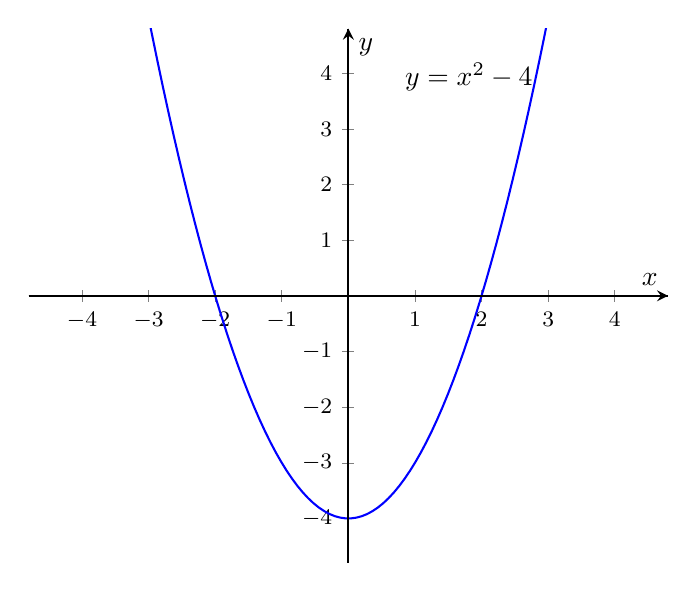
\begin{tikzpicture}
            \begin{axis}[
            width=0.8\textwidth,
            xlabel=$x$,
            ylabel=$y$,
            axis lines=middle,
            xmin=-4,
            xmax=4,
            ymin=-4,
            ymax=4,
            xtick={-4,-3,...,4},
            ytick={-4,-3,...,4},
            enlargelimits,
            ticks=both,
            %tick label style={font=\small}, % para diminuir o tamanho de fonte
            tick label style={font=\footnotesize}, % outra opção de tamanho de fonte
            % tick label style={font=\tiny} % é a menor fonte q tem
            after end axis/.code={
            \draw (axis cs:0,\pgfkeysvalueof{/pgfplots/ymin}) -- (axis cs:0,\pgfkeysvalueof{/pgfplots/ymax});
            \draw (axis cs:\pgfkeysvalueof{/pgfplots/xmin},0) -- (axis cs:\pgfkeysvalueof{/pgfplots/xmax},0);
            \node[black, above right] at (axis cs:0.7,3.5) {$y =x^2-4 $};
            %\node[black, below right] at (axis cs:-2.5,1) {$y =-x-2$};
            }
            ]
            \addplot[domain=-4:4, blue, samples=100] {x^2-4};
            %\addplot[domain=-3.5:0, Green, samples=100] {-x-2};
            \end{axis}
        \end{tikzpicture}
    \end{center}
            %%%%%%%%%%%%%%%%%%%%%%%%%%%%%%%%%%%%%%
            
        Assim, o gráfico de f(x)\\
            
             %%%%%%%%%%%%%%%%%%%%%%%%%%%%%%%%%%%%%%
    \begin{center}
        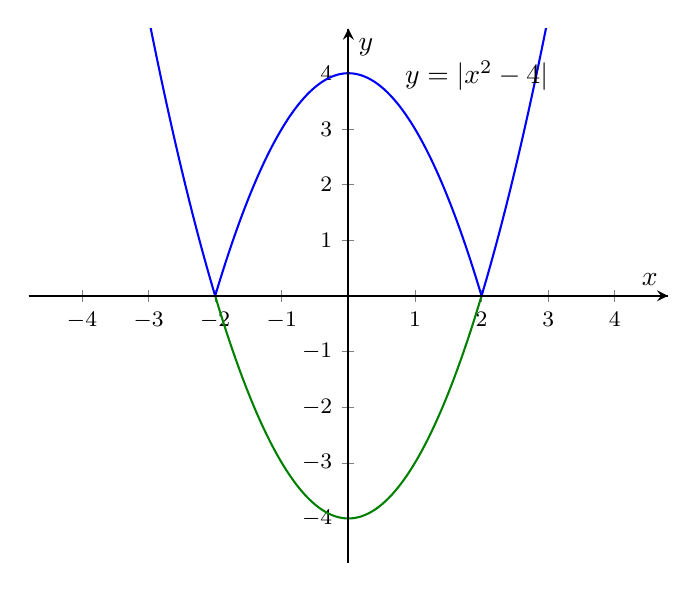
\begin{tikzpicture}
            \begin{axis}[
            width=0.8\textwidth,
            xlabel=$x$,
            ylabel=$y$,
            axis lines=middle,
            xmin=-4,
            xmax=4,
            ymin=-4,
            ymax=4,
            xtick={-4,-3,...,4},
            ytick={-4,-3,...,4},
            enlargelimits,
            ticks=both,
            %tick label style={font=\small}, % para diminuir o tamanho de fonte
            tick label style={font=\footnotesize}, % outra opção de tamanho de fonte
            % tick label style={font=\tiny} % é a menor fonte q tem
            after end axis/.code={
            \draw (axis cs:0,\pgfkeysvalueof{/pgfplots/ymin}) -- (axis cs:0,\pgfkeysvalueof{/pgfplots/ymax});
            \draw (axis cs:\pgfkeysvalueof{/pgfplots/xmin},0) -- (axis cs:\pgfkeysvalueof{/pgfplots/xmax},0);
            \node[black, above right] at (axis cs:0.7,3.5) {$y =|x^2-4| $};
            %\node[black, below right] at (axis cs:-2.5,1) {$y =-x-2$};
            }
            ]
            \addplot[domain=-4:-2, blue, samples=100] {x^2-4};
            \addplot[domain=2:4, blue, samples=100] {x^2-4};
            \addplot[domain=-2:2, blue, samples=100] {-x^2+4};
            \addplot[domain=-2:2, Green, samples=100] {x^2-4};
            \end{axis}
        \end{tikzpicture}
    \end{center}
            %%%%%%%%%%%%%%%%%%%%%%%%%%%%%%%%%%%%%%
            
    \end{enumerate}

    \section{Exercícios}
    
        \begin{enumerate}
	       \item (FUVEST) Seja $f(x)=|2x^2-1|, x \in \mathbb{R}$. Determine os valores de $x$ para os quais $f(x) < 1$ 
              \item Construa os gráficos das seguintes funções modulares:
	           \begin{tasks}
		          \task $f(x)=|x^2+4x|$
		          \task $f(x)=|4-x^2|$
                    \task $f(x)=|2x-1|$
		          \task $f(x)=|x-1|$
                    \task $f(x)=|2x+3|$
	           \end{tasks}
            \item Resolva a seguinte equação em $\mathbb{R}: |x-2| = 2x + 1$
            \item Resolva a seguinte inequação em $\mathbb{R}: |x-1| \le 3x - 7$
    \end{enumerate}

    \section{Respostas dos exercícios}
    
        \begin{enumerate}
	       \item $\{ x \in \mathbb{R} \mid -1 < x < 0 \text{ ou } o < x < 1 \} $.
              \item Construa os gráficos das seguintes funções modulares:
	           \begin{tasks}
		          \task 
            %%%%%%%%%%%%%%%%%%%%%%%%%%%%%%%%%%%%%%
    \begin{center}
        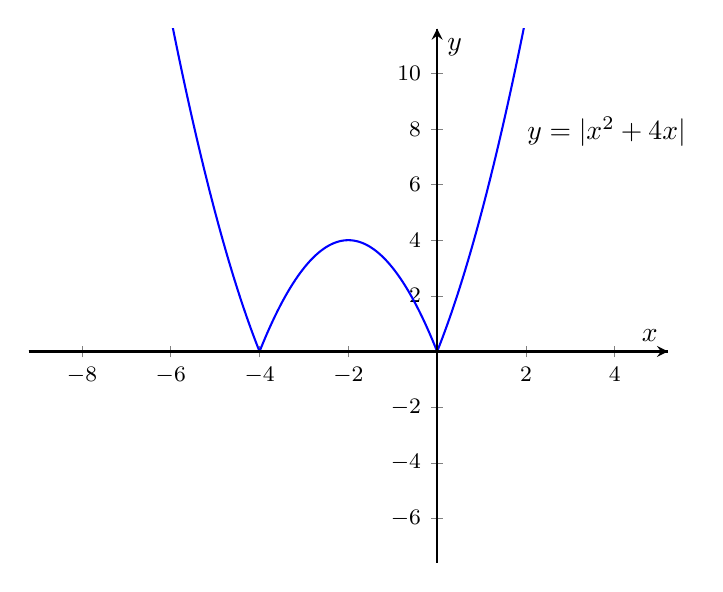
\begin{tikzpicture}
            \begin{axis}[
            width=0.8\textwidth,
            xlabel=$x$,
            ylabel=$y$,
            axis lines=middle,
            xmin=-8,
            xmax=4,
            ymin=-6,
            ymax=10,
            xtick={-8,-6,...,4},
            ytick={-6,-4,...,10},
            enlargelimits,
            ticks=both,
            %tick label style={font=\small}, % para diminuir o tamanho de fonte
            tick label style={font=\footnotesize}, % outra opção de tamanho de fonte
            % tick label style={font=\tiny} % é a menor fonte q tem
            after end axis/.code={
            \draw (axis cs:0,\pgfkeysvalueof{/pgfplots/ymin}) -- (axis cs:0,\pgfkeysvalueof{/pgfplots/ymax});
            \draw (axis cs:\pgfkeysvalueof{/pgfplots/xmin},0) -- (axis cs:\pgfkeysvalueof{/pgfplots/xmax},0);
            \node[black, above right] at (axis cs:1.8,7) {$y =|x^2+4x| $};
            %\node[black, below right] at (axis cs:-2.5,1) {$y =-x-2$};
            }
            ]
            %\addplot[domain=-4:-2, blue, samples=100] {x^2-4};
            \addplot[domain=0:4, blue, samples=100] {x^2+4*x};
            \addplot[domain=-8:-4, blue, samples=100] {x^2+4*x};
            \addplot[domain=-4:0, blue, samples=100] {-x^2-4*x};
            \end{axis}
        \end{tikzpicture}
    \end{center}
            %%%%%%%%%%%%%%%%%%%%%%%%%%%%%%%%%%%%%%
            
                    \task
            %%%%%%%%%%%%%%%%%%%%%%%%%%%%%%%%%%%%%%
    \begin{center}
        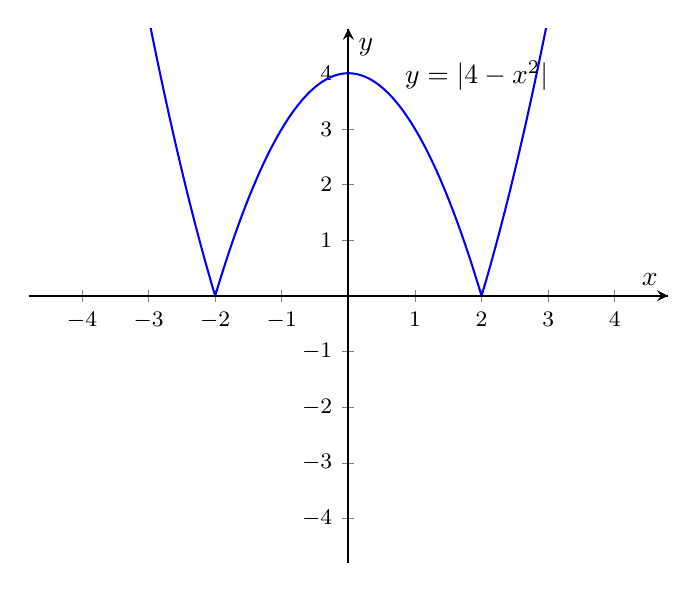
\begin{tikzpicture}
            \begin{axis}[
            width=0.8\textwidth,
            xlabel=$x$,
            ylabel=$y$,
            axis lines=middle,
            xmin=-4,
            xmax=4,
            ymin=-4,
            ymax=4,
            xtick={-4,-3,...,4},
            ytick={-4,-3,...,4},
            enlargelimits,
            ticks=both,
            %tick label style={font=\small}, % para diminuir o tamanho de fonte
            tick label style={font=\footnotesize}, % outra opção de tamanho de fonte
            % tick label style={font=\tiny} % é a menor fonte q tem
            after end axis/.code={
            \draw (axis cs:0,\pgfkeysvalueof{/pgfplots/ymin}) -- (axis cs:0,\pgfkeysvalueof{/pgfplots/ymax});
            \draw (axis cs:\pgfkeysvalueof{/pgfplots/xmin},0) -- (axis cs:\pgfkeysvalueof{/pgfplots/xmax},0);
            \node[black, above right] at (axis cs:0.7,3.5) {$y =|4-x^2| $};
            %\node[black, below right] at (axis cs:-2.5,1) {$y =-x-2$};
            }
            ]
            \addplot[domain=-4:-2, blue, samples=100] {x^2-4};
            \addplot[domain=2:4, blue, samples=100] {x^2-4};
            \addplot[domain=-2:2, blue, samples=100] {-x^2+4};
            %\addplot[domain=-2:2, Green, samples=100] {x^2-4};
            \end{axis}
        \end{tikzpicture}
    \end{center}
            %%%%%%%%%%%%%%%%%%%%%%%%%%%%%%%%%%%%%%
            
                    \task
            %%%%%%%%%%%%%%%%%%%%%%%%%%%%%%%%%%%%%%
    \begin{center}
        \begin{tikzpicture}
            \begin{axis}[
            width=0.8\textwidth,
            xlabel=$x$,
            ylabel=$y$,
            axis lines=middle,
            xmin=-3,
            xmax=3,
            ymin=-4,
            ymax=4,
            xtick={-3,-2,...,3},
            ytick={-4,-3,...,4},
            enlargelimits,
            ticks=both,
            %tick label style={font=\small}, % para diminuir o tamanho de fonte
            tick label style={font=\footnotesize}, % outra opção de tamanho de fonte
            % tick label style={font=\tiny} % é a menor fonte q tem
            after end axis/.code={
            \draw (axis cs:0,\pgfkeysvalueof{/pgfplots/ymin}) -- (axis cs:0,\pgfkeysvalueof{/pgfplots/ymax});
            \draw (axis cs:\pgfkeysvalueof{/pgfplots/xmin},0) -- (axis cs:\pgfkeysvalueof{/pgfplots/xmax},0);
            \node[black, above right] at (axis cs:0.7,3.5) {$y =|2x-1| $};
            %\node[black, below right] at (axis cs:-2.5,1) {$y =-x-2$};
            }
            ]
            \addplot[domain=0.5:3, blue, samples=100] {2*x-1};
            \addplot[domain=-3:0.5, blue, samples=100] {-2*x+1};
            %\addplot[domain=-2:2, blue, samples=100] {-x^2+4};
            %\addplot[domain=-2:2, Green, samples=100] {x^2-4};
            \end{axis}
        \end{tikzpicture}
    \end{center}
            %%%%%%%%%%%%%%%%%%%%%%%%%%%%%%%%%%%%%%
                    \task
            %%%%%%%%%%%%%%%%%%%%%%%%%%%%%%%%%%%%%%
    \begin{center}
        \begin{tikzpicture}
            \begin{axis}[
            width=0.8\textwidth,
            xlabel=$x$,
            ylabel=$y$,
            axis lines=middle,
            xmin=-2,
            xmax=4,
            ymin=-4,
            ymax=4,
            xtick={-2,-1,...,4},
            ytick={-4,-3,...,4},
            enlargelimits,
            ticks=both,
            %tick label style={font=\small}, % para diminuir o tamanho de fonte
            tick label style={font=\footnotesize}, % outra opção de tamanho de fonte
            % tick label style={font=\tiny} % é a menor fonte q tem
            after end axis/.code={
            \draw (axis cs:0,\pgfkeysvalueof{/pgfplots/ymin}) -- (axis cs:0,\pgfkeysvalueof{/pgfplots/ymax});
            \draw (axis cs:\pgfkeysvalueof{/pgfplots/xmin},0) -- (axis cs:\pgfkeysvalueof{/pgfplots/xmax},0);
            \node[black, above right] at (axis cs:1.7,2) {$y =|x-1| $};
            %\node[black, below right] at (axis cs:-2.5,1) {$y =-x-2$};
            }
            ]
            \addplot[domain=1:4, blue, samples=100] {x-1};
            \addplot[domain=-2:1, blue, samples=100] {-x+1};
            %\addplot[domain=-2:2, blue, samples=100] {-x^2+4};
            %\addplot[domain=-2:2, Green, samples=100] {x^2-4};
            \end{axis}
        \end{tikzpicture}
    \end{center}
            %%%%%%%%%%%%%%%%%%%%%%%%%%%%%%%%%%%%%%
                    \task
            %%%%%%%%%%%%%%%%%%%%%%%%%%%%%%%%%%%%%%
    \begin{center}
        \begin{tikzpicture}
            \begin{axis}[
            width=0.8\textwidth,
            xlabel=$x$,
            ylabel=$y$,
            axis lines=middle,
            xmin=-5,
            xmax=3,
            ymin=-4,
            ymax=4,
            xtick={-5,-4,...,3},
            ytick={-4,-3,...,4},
            enlargelimits,
            ticks=both,
            %tick label style={font=\small}, % para diminuir o tamanho de fonte
            tick label style={font=\footnotesize}, % outra opção de tamanho de fonte
            % tick label style={font=\tiny} % é a menor fonte q tem
            after end axis/.code={
            \draw (axis cs:0,\pgfkeysvalueof{/pgfplots/ymin}) -- (axis cs:0,\pgfkeysvalueof{/pgfplots/ymax});
            \draw (axis cs:\pgfkeysvalueof{/pgfplots/xmin},0) -- (axis cs:\pgfkeysvalueof{/pgfplots/xmax},0);
            \node[black, above right] at (axis cs:1.7,2) {$y =|2x+3| $};
            %\node[black, below right] at (axis cs:-2.5,1) {$y =-x-2$};
            }
            ]
            \addplot[domain=-1.5:3, blue, samples=100] {2*x+3};
            \addplot[domain=-5:-1.5, blue, samples=100] {-2*x-3};
            %\addplot[domain=-2:2, blue, samples=100] {-x^2+4};
            %\addplot[domain=-2:2, Green, samples=100] {x^2-4};
            \end{axis}
        \end{tikzpicture}
    \end{center}
            %%%%%%%%%%%%%%%%%%%%%%%%%%%%%%%%%%%%%%
	           \end{tasks}
            \item 
            $S=\left\{ \dfrac{1}{3}\right\}$
            \item 
            $S=\{ x \in \mathbb{R} \mid x \ge 3 \}$
    \end{enumerate}